\section{Performances attendues du sous-système FLIR intégré au système de vision en réalité augmentée}\label{partie1}

\begin{obj}
Déterminer les performances de rapidité et de précision d'orientation de la ligne de visée du sous-système
FLIR qui permettent de satisfaire le cahier des charges du système de vision en réalité augmentée
pour hélicoptère.
\end{obj}

\subsection{Validation des performances simulées du FLIR}

Le sous-système de détection de posture, appelé \textit{DDP}, placé sur le casque TopOwl permet d'acquérir l'orientation
spatiale de la tête du pilote par rapport au cockpit du porteur (3 angles de rotation). Cette information, couplée
à l'information de position et d'orientation du porteur par rapport à la Terre (délivrée par une centrale inertielle fixée au porteur), permet d'élaborer la commande d'orientation du FLIR afin que sa ligne de visée corresponde
à la ligne de visée du pilote. À partir d'un algorithme, une centrale de traitement d'image permet de calculer
l'image à afficher sur la visière du casque TopOwl et les informations éventuelles à ajouter, comme celles issues
de la position GPS par exemple.

\subsection{Détermination des performances du FLIR}

Le système de détection de posture (DDP) a besoin d'un temps noté $\indice{t}{ddp}$ égal à $\SI{20}{ms}$ pour acquérir l'information. De même, le temps de traitement de l'information par filtrage noté $\indice{t}{filtre}$ est égal à $\SI{5}{ms}$.
On donne les temps suivants pour la réalisation des tâches :
\begin{itemize}
\item les temps d'acquisition des informations par les capteurs autres que la DDP sont négligeables devant les
autres temps ;
\item le temps d'acquisition de l'image par les caméras du FLIR est négligeable devant les autres temps ;
\item le temps de traitement des informations issues des caméras du FLIR (traitement des images) est noté
$\indice{t}{trait}$ = 50 ms maximum ;
\item le temps mis par le TopOwl pour afficher l'image est noté $\indice{t}{com} = 5 ms$.
\end{itemize}

\begin{figure}[!htb]
\begin{center}
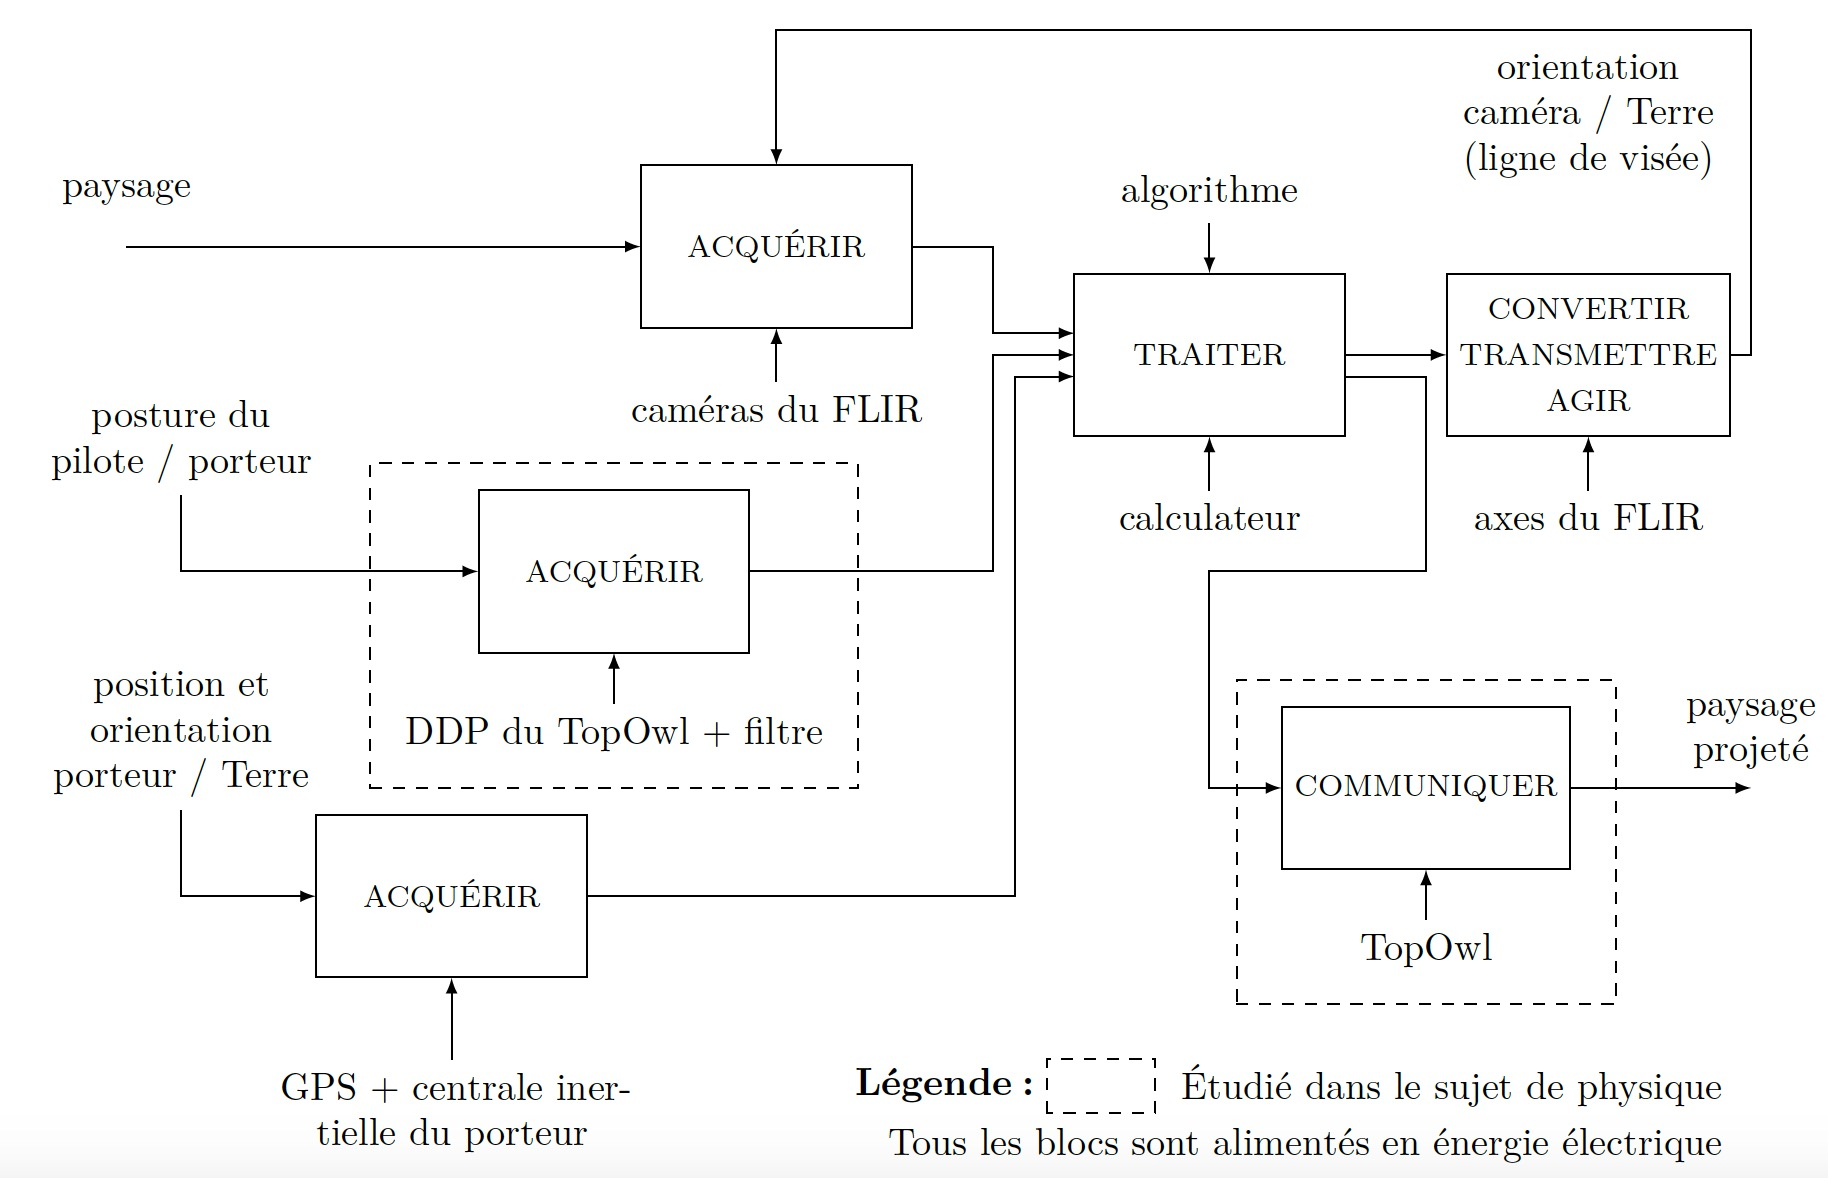
\includegraphics[width=0.9\textwidth]{chaine_fonctionnelle3.jpg}
\caption{Description structuro-fonctionnelle du système de vision en réalité augmentée \label{chaine_fonctionnelle}}
\end{center}
\end{figure}

\question{À l'aide de la description structuro-fonctionnelle de la figure \ref{chaine_fonctionnelle}, déterminer littéralement et numériquement
en fonction des données précédentes le temps maximal disponible pour orienter les caméras du FLIR, noté
$t_{disponible}$, qui permet de vérifier le troisième critère de l'exigence 1.1.}

\begin{figure}[!htb]
\begin{center}
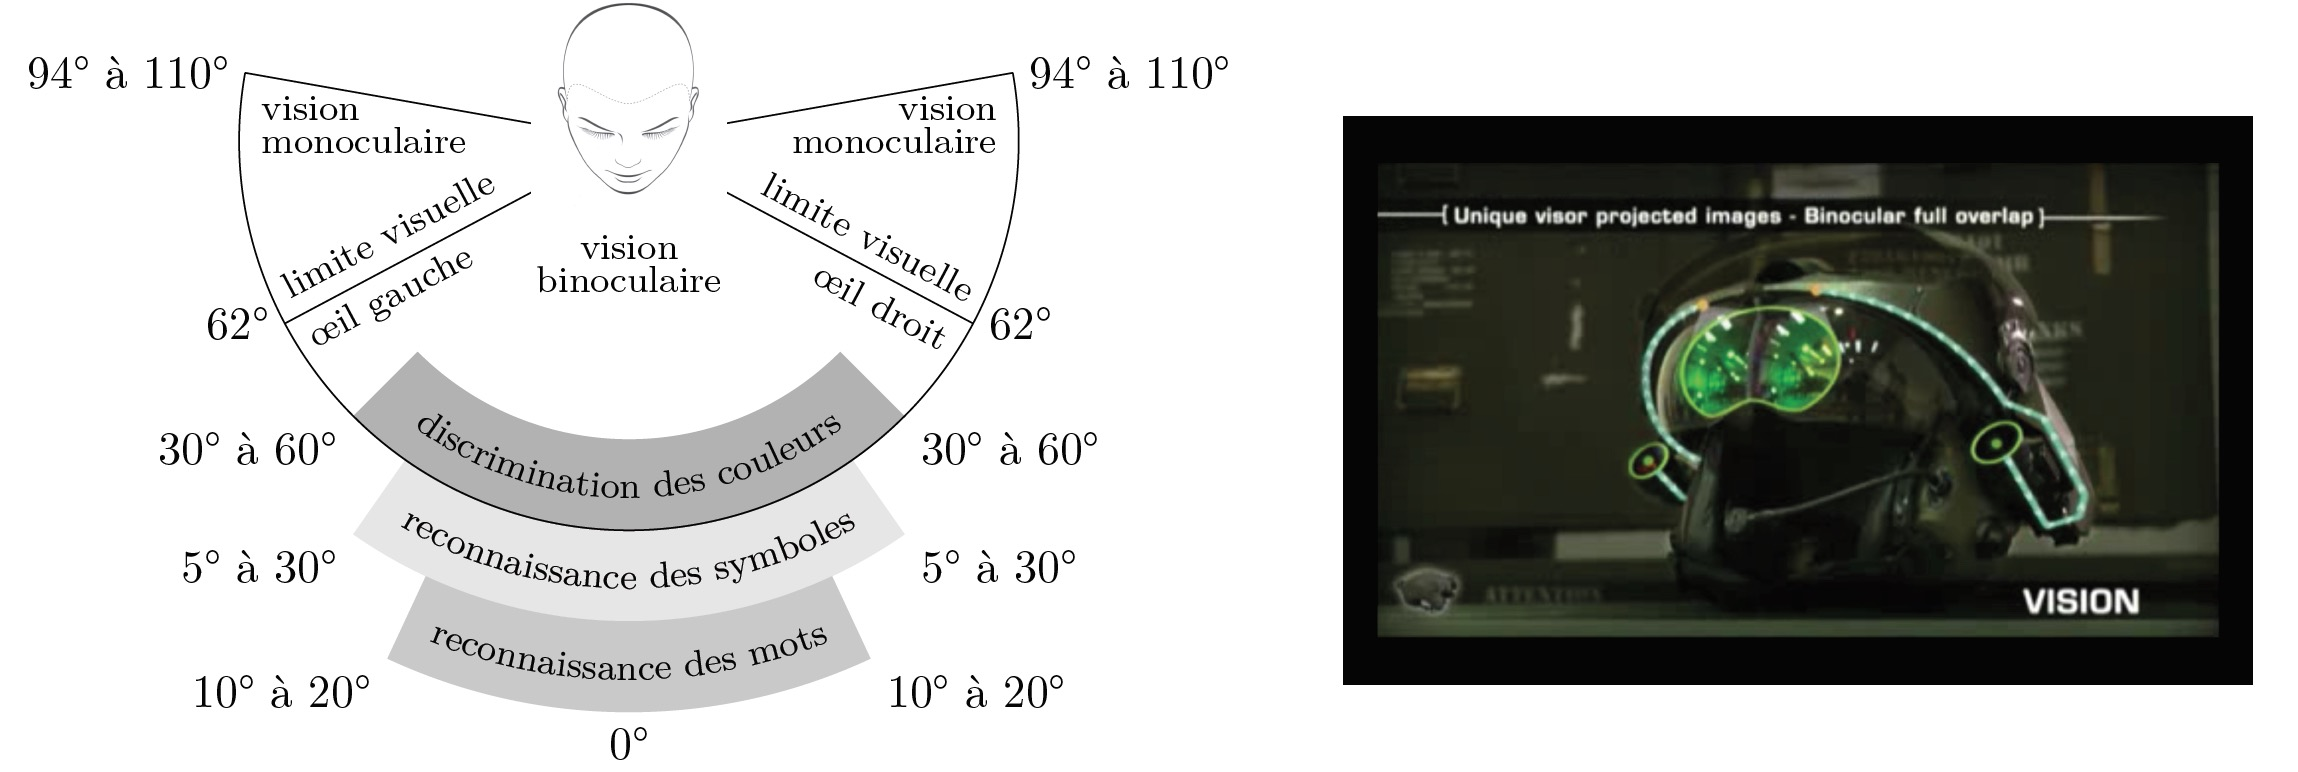
\includegraphics[width=0.9\textwidth]{figure6.jpg}
\caption{Champ de vision humain et projection des deux images sur la visière \label{figure6}}
\end{center}
\end{figure}

Le format choisi correspond à une image rectangulaire de 1024 pixels de large et 768 pixels de haut. Cette image
est projetée deux fois sur la visière, une projection pour chaque oeil du pilote. Les deux projections se chevauchent
entièrement (Binocular full overlap). La visière se trouve à 5 cm des yeux du pilote et chaque image est projetée
de façon à occuper entièrement le champ de vision le plus large possible permettant la reconnaissance des mots.

\question{Calculer à partir des informations précédentes et de la figure \ref{figure6} la largeur d'un pixel (en mm) projeté sur
la visière. Conclure quant au respect du critère de résolution d'affichage de l'exigence 1.1.}

\question{Déterminer l'écart angulaire maximal admissible, exprimé en rad, entre la ligne de visée du pilote et la
ligne de visée des caméras qui permet de respecter le critère de précision de l'exigence 1.1.}


Afin de vérifier les performances du FLIR qui viennent d'être déterminées, et compte tenu de son niveau de
complexité élevé, il est nécessaire d'émettre et de valider des hypothèses simplificatrices de modélisation relatives
à son comportement.
